\section{Introduction}

In this Chapter, we describe the semantics and mechanisms that our programming abstraction builds upon, which enable developers to decide \textbf{what} and \textbf{where} data are collected and analyzed. 

Publish/subscribe (pub/sub) systems are widely used in IoT applications such as environment monitoring, supply chain tracing, healthcare, and vehicle networks. The Publish Subscribe model enables event-driven architectures and asynchronous parallel processing, while improving performance, reliability and scalability. Pub/sub protocols, however, make some common task in IoT more challenging to achieve, for instance, it is not straightforward to discover potential publishers of a particular type or in a particular location. The lack of publisher and subscriber discovery is a key challenge that has to be overcome to enable the interoperability of different IoT data providers and producers. For those reasons we chose the Associative Rendezvous (AR), a paradigm for content-based decoupled interactions with programmable reactive behaviors.  AR allows highly expressive descriptions . AR differs from the traditional publish/subscribe paradigms in that it does not relay in topics, it relays on well defined combinations of keywords (i.e.keywords, partial keywords, wildcards, ranges) from a semantic information space to defined the properties of the publisher or subscriber.

Rendezvous-based interactions~\cite{AR} provide a mechanism for decoupling senders and receivers. The Rendezvous Point (RP) is the node where rendezvous interactions occur, and it can be an edge node or a cloud node. Senders transmit messages to an RP without knowledge of who or where the receivers are. The associative rendezvous interaction model consists of three elements, messages, associative selection, and reactive behaviors, which are described below. In the following sections we will first describe the semantics and primitives of AR and then we present the adaptation of AR semantics and primitives to fit our model. The R-Pulsar AR approach is an adaptation of existing primitives from Meteor~\cite{meteor2008}.

\section{Associative Rendezvous} 
Associative Rendezvous is a paradigm for content-based decoupled interactions with programmable reactive behaviors. Rendezvous-based interactions~\cite{AR} provide a mechanism for decoupling senders and receivers. The Rendezvous Point (RP) is the node where rendezvous interactions occur, and it can be an edge node or a cloud node. Senders transmit messages to an RP without knowledge of who or where the receivers are. The associative rendezvous interaction model consists of three elements, messages, associative selection, and reactive behaviors, which are described below. The AR interaction model consists of three elements: messages, associative selection, and reactive behaviors, which are described below~\cite{meteor2008}.

\begin{figure}
    \centering
    \begin{subfigure}[t]{0.5\textwidth}
        \centering
        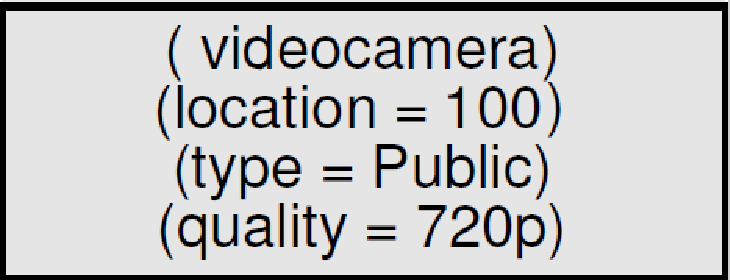
\includegraphics[height=1in]{Figures/data_profile.pdf}
        \caption{}
        \label{fig:data_profile}
    \end{subfigure}%
    ~ 
    \begin{subfigure}[t]{0.5\textwidth}
        \centering
        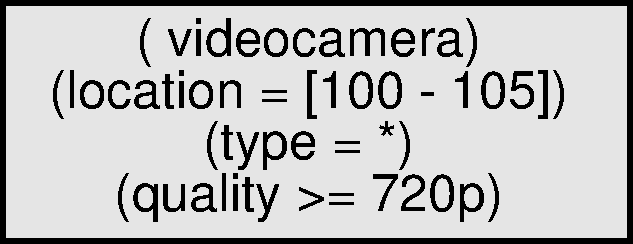
\includegraphics[height=1in]{Figures/interest_profile.pdf}
        \caption{}
        \label{fig:interest_profile}
    \end{subfigure}
    \caption{Sample profiles: (a) producer profile from a video camera sensor; (b) consumer profile interested in video camera sensors}\label{fig:samples_profiles}
\end{figure}



\subsection{AR Message}
An AR message~\cite{meteor2008} is defined as the triplet: (header, action, data). The data field may be empty or may contain the message payload. The header includes a semantic profile in addition to the credentials of the sender, a message context, and the Lifetime of the message. The profile is a set of attributes and/or attribute–value pairs, and defines the set of recipients of the message. The attributes are keywords from the application information space, such as the type of data a sensor produces (temperature or humidity) and/or its location, the type of functionality a service provides and/or its quality of service guarantees, and the capability and/or the cost of a resource, while the values field may be a keyword, partial keyword, wildcard, or range from the same space. At the RP, a profile is classified as a data profile or an interest profile depending on the action field of the message. The data profile corresponds to a message carrying data to be stored in the system. The interest profile corresponds to a query.

\subsection{Associative Selection} 

Profiles are represented using a hierarchical schema that can be efficiently stored and evaluated by the selection engine at runtime. Profile $p$ represents a path in the hierarchical schema, [$e_0$ $\bigtriangleup$ ... $e_k$], where $e_i$ is an element operand and $\bigtriangleup$ can be a parent-child ("/") operator (i.e. at adjacent levels) or an ancestor-descendant ("//") operator (i.e. separated by more than one level). Within a level, the profile defines a propositional expression where $\bigtriangleup$ represents propositional operators, such as $\wedge$ and $\vee$ between elements at the same level. Note that the propositional expression at a level must be evaluated as TRUE for the evaluation to continue to the next level. The elements of the profile can be an attribute, $e_i$ : ($a_i$), or an attribute-value pair $e_i$ : ($a_i$, $v_i$), where $a_i$ is a keyword and $v_i$ may be a keyword, partial keyword, wildcard, or range. The singleton attribute $a_i$ evaluates to true if and only if $p$ contains the simple attribute $a_i$. The attribute-value pair ($a_i$,$u_i$) evaluates to true with respect to a profile $p$, if and only if $p$ contains attribute $a_i$ and the corresponding value $v_i$ satisfies $u_i$. For example, the profile in Figure~\ref{fig:data_profile} will be matched by the profile in Figure~\ref{fig:interest_profile}, since (1) both have matched singleton attribute video camera; (2) for attribute location, 100 - 105, satisfies the range relation; (3) for attribute type, {\it Public} matches the wildcard *; and (4) quality$=$720p satisfies the request quality$>=$720p. 
\\
\begin{table}[h]
\caption{AR Reactive behaviors}
\label{table:OldActions}
\begin{adjustwidth}{-1cm}{-1cm}

\begin{tabular}{ll}
\hline
\textbf{Actions} & \textbf{Semantics}                                                                                                                                                                                                                 \\ \hline
store            & \begin{tabular}[c]{@{}l@{}}Store data profile and data in the system at the RPs\\ Match the data profile with existing interest profiles with 'notify data' action\\ Execute action associated with a matched profile\end{tabular} \\ \hline
retrieve         & \begin{tabular}[c]{@{}l@{}}Match interest profile with existing data profiles\\ Send data associated with the matched profiles to the requester\end{tabular}                                                                       \\ \hline
notify\_data     & Match message profile with existing data/interest profiles.                                                                                                                                                                        \\
notify\_interest & Notify sender if there is at least one match.                                                                                                                                                                                      \\
delete\_data     & Match message profile with existing data/interest profile.                                                                                                                                                                         \\
delete\_interest & \begin{tabular}[c]{@{}l@{}}Notify sender if there is at least one match.\\ Remove all matching data/interest profiles from the system.\end{tabular}                                                                                \\ \hline
\end{tabular}
\end{adjustwidth}
\end{table}

\subsection{Reactive Behaviors} 

The action field of the message defines the reactive behavior of the profile when a match occurs. Every time an RP receives an AR message, the profile is stored and matched against existing profiles. If there is a match, the action of the profile is carried out. Basic reactive behaviors are store, retrieve, notify, and delete. Table~\ref{table:OldActions} summarizes the available actions.

The notify and delete actions are explicitly invoked on a data or an interest profile. The store action stores the data and data profile at the RP. It also causes the message profile to be matched against existing interest profiles with notify data action, and the data to be sent to the data consumers that requested it in case of a positive match.

The retrieve action retrieves data corresponding to each matching data profile. The notify action matches the message profile against existing interest/data profile, and notifies the sender if there is at least one positive match. 

The notify action comes in two flavors: notify data and notify interest. Notify data is used by data consumers, who want to be notified when data matching their interest profile are stored in the system. Notify interest can be used by data producers, who want to be notified when there is interest in the data they produce, so that they can start sending data into the system.

Finally, the delete action deletes all matching interest/data profiles. Note that the actions will only be executed if the message header contains an appropriate credential. Also note that each message is stored at the rendezvous for a period corresponding to the Lifetime defined in its header. In case of multiple matches, the profiles matching are processed in random order.

\section{R-Pulsar Associative Rendezvous}\label{sec:semantics}
R-Pulsar uses a custom implementation of the original AR semantics~\cite{meteor2008}. In our new implementation of the AR model, we modified to elements: the AR Message and the Reactive Behaviors.

The AR message is now defined as a quintuplet instead of the original triplet: (header, action, data, location, and data-processing task). The location and data processing task fields have been added in to the already existing fields. The location field has been added so the AR message can be routed based on the location and the content, where the original version of AR only routes messages based on the content. The location coordinates represent the physical location of the sensors or the physical location of where to deploy data-processing tasks and the tag helps decide where to deploy data-processing tasks, either the edge or the cloud, allowing to pick from multiple cloud or edge geographically distributed resources.

\begin{table}[t]
\caption{R-Pulsar Reactive behaviors}
\label{table:actions}
\begin{adjustwidth}{0cm}{-1cm}
\begin{tabular}{ll}
\hline
\textbf{Actions} & \textbf{Semantics}                                                                                                                                  \\ \hline
store            & Store data in rendezvous point queue.                                                                                                               \\ \hline
profiles         & \begin{tabular}[c]{@{}l@{}}Notify sender all the interest\_profiles stored in that rendezvous\\ point.\end{tabular}                                 \\ \hline
store\_topology  & Store the new topology in the RP.                                                                                                                   \\
start\_topology  & Start the topology in the RP.                                                                                                                       \\
stop\_topology   & Stop the topology.                                                                                                                                  \\
delete\_topology & Delete the topology.                                                                                                                                \\ \hline
notify\_data     & Match message profile with existing data/interest profiles.                                                                                         \\
notify\_interest & Notify sender if there is at least one match.                                                                                                       \\
query\_data      & Allows to perform SQL-like queries on stored data.                                                                                                  \\
delete\_data     & Match message profile with existing data/interest profile.                                                                                          \\
delete\_interest & \begin{tabular}[c]{@{}l@{}}Notify sender if there is at least one match.\\ Remove all matching data/interest profiles from the system.\end{tabular} \\ \hline
\end{tabular}
\end{adjustwidth}
\end{table}

For the reactive behaviors are now classified in two two different classes: resource actions and function actions. Where in the original implementation of AR there where only one type of actions. Table~\ref{table:actions} summarizes the available actions.

Resource actions are designated for discovering, starting, and stopping sensors from transmitting data. Basic resource reactive behaviors currently defined include {\it notify\_interest, notify\_data, query\_data}, and {\it delete}. The {\it notify\_interest} is used by sensors for advertising its data producing capabilities and that they want to be notified when there is someone interested in the data they can produce. The {\it notify\_data} are used by the data-processing tasks that will consume the data produced by sensors. When a {\it notify\_data} profile and a {\it notify\_interest} profile match, Figure~\ref{fig:samples_profiles} sensors are notified to start streaming data to the consumer. The {\it query\_data } action is for performing SQL-like queries on stored data. The {\it delete} action deletes all matching profiles from the system.

Function actions are designated for storing, triggering, and stopping data-processing tasks. Basic function reactive behaviors currently defined include {\it store\_function, start\_function and stop\_function}. The {\it store\_function} action allows users to submit and store user-defined data-processing tasks in the RPs, allowing to share and discover existing data-processing tasks previously uploaded by other users. This avoids the need to rewrite the same function multiple times and facilitates the reproducibility of the experiments. The {\it start\_function} allows users to trigger data-processing tasks on demand. If there is a match between two profiles, the data-processing task is executed. The {\it stop\_function} allows users to stop data-processing tasks that are running. 

\subsection{Illustrative Example}

This section illustrates two operation examples of the R-Pulsar AR model. The first example in Figure~\ref{fig:ARExample} illustrates the exchange of messages for subscribing to sensors in R-Pulsar. The second example in Figure~\ref{fig:AR-Multi} demonstrates the one-to-many interactions using the R-Pulsar associative rendezvous.

\begin{figure}[h]
\centering
\begin{subfigure}[b]{0.8\textwidth}
   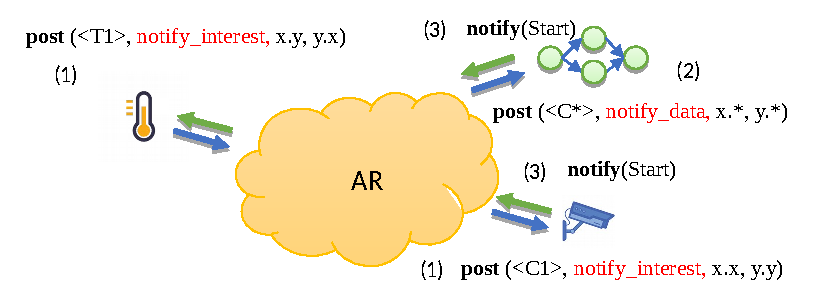
\includegraphics[width=1.1\linewidth]{Figures/AR_Exmple_1.pdf}
   \caption{}
\end{subfigure}
\begin{subfigure}[b]{0.8\textwidth}
   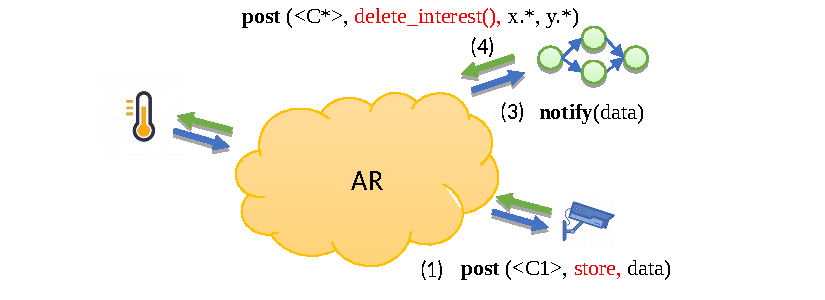
\includegraphics[width=1.1\linewidth]{Figures/AR_Example_2.pdf}
   \caption{}\label{fig:ARExample2} 
\end{subfigure}
\caption{An example illustrating the operation of associative rendezvous.}\label{fig:ARExample} 
\end{figure}

For this example we have two different types of data producers/sensors in this case we have a temperature sensors and a CCTV camera as data producers. In step (1) both sensors perform is to register themselves into the system by advertising the type of data they can produce and where they are located, in the case of the temperature sensor its described by the profile $<T1>$, x.y,y.x and $<C1>$ x.x, y.y for the CCTV camera. By doing that they are requesting to be notified if there are other clients interested in the type of data that they can produce. Both interest profiles are stored in the system, and matched against existing interest profiles. Since there is no interest profiles stored in the system nothing else happens. Both data producers/sensors publishes data in the system only if other clients need it. In step (2) the data consumer/computation is interested in consuming a very specific type of data, in this case it is interested in consuming data that matches the profile $<C*>$ and it is located in x.*,y.*.,  requesting to be notified if there are data stored in the system matching the profile. The interest profile of the computation is stored in the system and matched against the other profiles in the system. Since the notify data profile matches the profile of the CCTV camera, in step (3) a notification message is sent to the CCTV camera that someone is interested in its data and to start pushing the data into the system. In Figure~\ref{fig:ARExample2} step (4) the camera starts publishing data in the system, the data published by the camera matches the data profile specified by the computation,  resulting in step (5) the data being send to the computation for processing. After a few minutes the computation decide that the data the CCTV camera is producing is no longer valuable and decides the unsubscribe from it by sending a delete interest in step (6), pushing a notification to the CCTV camera to sop pushing data to the system.

\begin{figure}[h!]
  \centering
  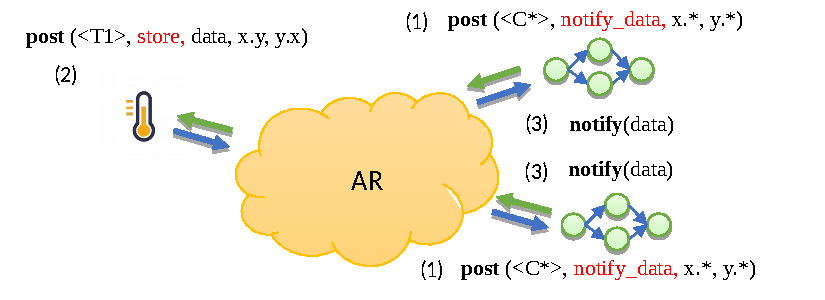
\includegraphics[width=0.8\textwidth]{Figures/AR_Example_Multi.pdf}
  \caption{One-to-many interactions using associative rendezvous.}
  \label{fig:AR-Multi}
\end{figure}

AR can also be used to realize different interaction semantics such as one-to-many, one-to-some and one-to-all. Figure~\ref{fig:AR-Multi} illustrates a one-to-many (e.g. multicast) interaction using AR. The example assumes that the temperature sensor has already been registered in the system with the notify interest profile $<T1>$. In step (1) the two data consumers register in the system requesting to be notified if there are data stored in the system matching the profile. In step (2) the interest profile of the computation is stored in the system and matched against the other profiles in the system. Since the notify data profile matches the profile of the temperature sensor, a notification message is sent to the temperature sensor that someone is interested in its data and to start pushing the data into the system. In step (3) the temperature sensor published data into the system. In step (4) the data published by the sensor matches the notify data profile of the two consumers so both consumers are notified with the data.